%\title{Reporte de reporte 1}
\documentclass[12pt,letterpaper]{article}     % Tipo de documento y otras especificaciones
\usepackage[utf8]{inputenc}                   % Para escribir tildes y eñes
\usepackage[spanish]{babel}                   % Para que los títulos de figuras, tablas y otros estén en español
\addto\captionsspanish{\renewcommand{\tablename}{Tabla}}					% Cambiar nombre a tablas
%\addto\captionsspanish{\renewcommand{\listtablename}{Índice de tablas}}		% Cambiar nombre a lista de tablas
\usepackage{geometry}                         
\geometry{left=18mm,right=18mm,top=21mm,bottom=21mm} % Tamaño del área de escritura de la página
\usepackage{ucs}
\usepackage{amsmath}      % Los paquetes ams son desarrollados por la American Mathematical Society
\usepackage{amsfonts}     % y mejoran la escritura de fórmulas y símbolos matemáticos.
\usepackage{amssymb}
\usepackage{graphicx}     % Para insertar gráficas
\usepackage[lofdepth,lotdepth]{subfig}	% Para colocar varias figuras
\usepackage{unitsdef}	  % Para la presentación correcta de unidades
\usepackage{pdfpages}   %incluir paginas de pdf externo, para los anexos
\usepackage{appendix}   %para los anexos
\renewcommand{\unitvaluesep}{\hspace*{4pt}}	% Redimensionamiento del espacio entre magnitud y unidad
\usepackage[colorlinks=true,urlcolor=blue,linkcolor=black,citecolor=black]{hyperref}     % Para insertar hipervínculos y marcadores
\usepackage{float}		% Para ubicar las tablas y figuras justo después del texto
\usepackage{booktabs}	% Para hacer tablas más estilizadas
\batchmode
\bibliographystyle{plain} 
\pagestyle{plain} 
\pagenumbering{arabic}
\usepackage{lastpage}
\usepackage{fancyhdr}	% Para manejar los encabezados y pies de página
\pagestyle{fancy}		% Contenido de los encabezados y pies de pagina
\usepackage{multicol}   % Para varias columnas

%---------------------------Definición del environment resumen---------------------------
\newcounter{resumen}
\setcounter{resumen}{0}
\def\theejemplo{\thechapter.\arabic{resumen}}

\newenvironment{resumen}
{	
	\begin{center}
	\begin{minipage}[t]{500 pt}
	\vspace{5mm}
	\emph{\textbf{Resumen}}
	\\[-2mm]
	\line(1,0){500}
	\\[-4.25 mm]
	\line(1,0){500}
	\\
}
{
	\normalsize
	\\[2mm]
	\footnotesize\textbf{Palabras clave: \footnotesize\@palabras}
	\\[-2mm]
	\line(1,0){500}
	\\[0.5cm]
	\end{minipage}
	\end{center}
}

% -------------------- Para las palabras clave -------------- %
\def\palabras#1{\gdef\@palabras{#1}}

%%%%%%%%%%%%%%%%%%%%%%%%%%%%%%%%%%%%

\lhead{Control I}
\chead{}
\rhead{Polos y Ceros encontrados por Inspección}	% Aquí va el numero de experimento, al igual que en el titulo
\lfoot{Departamento de Ingeniería electrónica}
\cfoot{\thepage\ de \pageref{LastPage}}
\rfoot{Tecnológico Nacional de México}


\author{Luz Vanessa Pacheco Medina, 14121133 \\ Martha Yepez Chavez, 12121166 \\ {\small Grupo A}\\ Profesor: Gerardo Marx Chávez Campos  \vspace*{3.0in}}
\title{Tecnólogico Nacional de México\\Instituto Tecnológico de  Morelia\\{\small Departamento de Ingeniería Electrónica\\Control I\\\vspace*{0.55in} Reporte De Laboratorio}\\ Polos y Ceros Encontrados por Inspección \vspace*{1.35in}}
\date{27 de noviembre del 2017}  				

%%%%%%%%%%%%%%%%% PALABRAS CLAVE 
%\palabras{LateX, TINA, Filtros Pasivos}
%%%%%%%%%%%%%%%%%
% Se escriben después del resumen y sintetizan los conceptos fundamentales del experimento a modo de etiquetas


%%%%%%%%%%%%%%%%
\begin{document}	% Inicio del documento
%%%%%%%%%%%%%%%%

\pdfbookmark[1]{Portada}{portada} 	% Marcador para el título

\maketitle							% Título


\tableofcontents
\newpage
\listoffigures
%\listoftables

\newpage
\section{Introducción}
%%%%%%%%%%%%%%%%%%%
En matemáticas polos y ceros es un método que permite evaluar los polos y los ceros  de las expresiones racionales  para hallar el conjunto solución en desigualdades. Su utilidad radica en la generalización y mecanización del proceso.Un sistema es estable si la respuesta del impulso tiende a cero, se puede decir que el sistema es críticamente o marginablemente estable.Una magnitud infinita hace el sistema inestable.
\begin{figure}[h!]
\centering
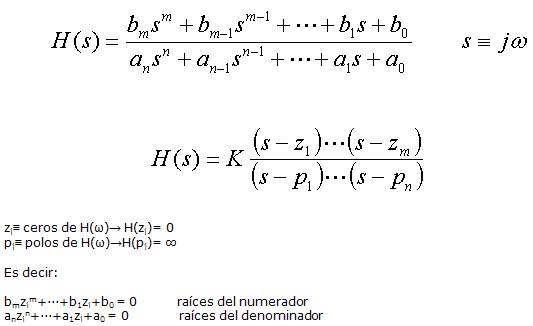
\includegraphics[width=3in]{Polos}
\caption{Relación de una función de transferencia con polos y ceros}
\end{figure}
\\
1.-Si todos los polos de la función de transferencia están  en el lado izquierdo del plano-s entonces el sistema es estable.
\\
2.- Un sistema es críticamente estable si uno o más polos están en el eje imaginario del plano-s.
\\
3.-Los polos de un sistema son las raíces obtenidas de el denominador de la función de transferencia cuando es igualado a cero (Polinomio característico).
\\
4.-El concepto de estabilidad es aplicado a sistemas a lazo cerrado o lazo abierto.
%%%%%%%%%%%%%%%%%%%

\section{Material utilizado} 
\begin{itemize}
	\item Osciloscopio
	\item Generador de funciones
	\item etc.
\end{itemize}
-Osciloscopio digital.\\
-Generador de funciones.\\
-Inductor  6.77mH.\\
-Resistencias 1k, 10k.

%%%%%%%%%%%%%%%%%%%
\section{Metodología}
%%%%%%%%%%%%%%%%%%%

\begin{figure}[h!]
\centering
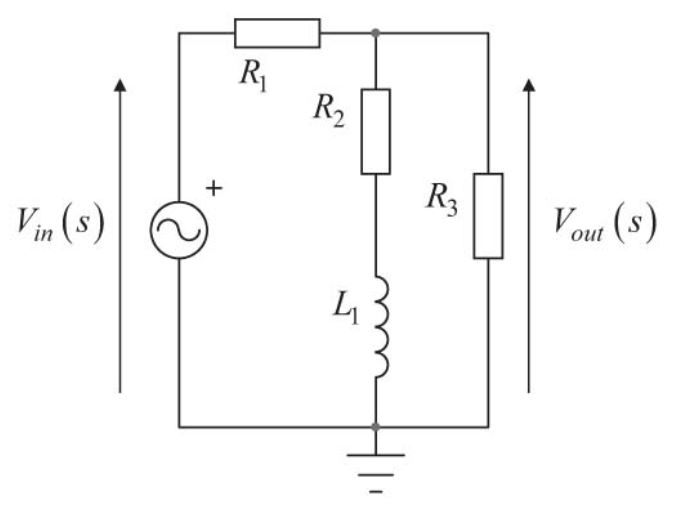
\includegraphics[width=3in]{Circuito}
\caption{Sistema eléctrico para analizar.}

\end{figure}

1.-Para la parte uno se obtiene la función de transferencia bajo inspección del siguiente circuito.
\\
Se obtiene la siguiente representación para le función de transferencia :

\begin{equation}\label{eq:ej1}
V_{out}(S) = G_{0}\frac{(1+S/W_{z1})}{(1+S/W_{p1})} 
\end{equation}
\\\\\\
Donde:
\\
G0=Atenuación en DC.\\
EL numerador: Son los ceros.\\
El denominador: Son los polos.\\\\
Se cierra el inductor ya que S=0, por lo tanto se tiene que G0 es:

\begin{equation}\label{eq:ej2}
Z_{L} = SL = 0
\end{equation}

\begin{equation}\label{eq:ej3}
V_{out}(S) = V_{in}(S)\frac{\frac{R_{3}R_{2}}{R_{3}+R_{2}} }{\frac{R_{3}R_{2}}{R_{3}+R_{2}}+R_{1}}
\end{equation}
se obtienen los ceros del sistema:
\begin{equation}\label{eq:ej4}
R_{2}+SL=0
1+ \frac{SL}{R_{2}}  =0
\end{equation}
Se obtiene la parte de los polos encontrando la Requivalente y Tau de una bobina.
\begin{equation}\label{eq:ej5}
R_{Eq} = \frac{1 }{\frac{R_{1}R_{3}}{R_{3}+R_{1}}+R_{2}}
\end{equation}
Si se tiene que Tau=L/R:
\begin{equation}\label{eq:ej6}
W_p1=\frac{L }{\frac{R_{1}R_{3}}{R_{3}+R_{1}}+R_{2}}
\end{equation}
Finalmente se obtiene la función de transferencia:
\begin{equation}\label{eq:ej7}
H(S) = \frac{R_{2}R_{3} }{R_{3}R_{2}+R_{1}(R_{3}+R_{1})} \frac{1+\frac{LS}{R_{2}}}{\frac{LS}{R_{1}||R_{3}+R_{2}}+1}
\end{equation}

2.-Obtener la FT (Alta entropía) usando métodos comunes de álgebra

Se hace un divisor de voltaje para obtener el voltaje de salida:

\begin{equation}\label{eq:ej8}
H(S) = \frac{(R_{2}+LS)R_{3}}{(R_{2}+LS)||R_{3}+R_{1}}
\end{equation}
Se reduce la expresión y se factoriza el G0:
\begin{equation}\label{eq:ej9}
H(S) = \frac{R_{2}R_{3} }{R_{3}R_{2}+R_{1}(R_{3}+R_{1})} \frac{1+\frac{LS}{R_{2}}}{\frac{R_{3}R_{2}+R_{3}SL+R_{1}R_{3}+R_{1}R_{2}+R_{1}SL}{R_{2}R_{3}+R_{1}R_{2}+R_{1}R_{3}}}
\end{equation}
Se reducen los términos
\begin{equation}\label{eq:ej9}
H(S) = \frac{R_{2}R_{3} }{R_{3}R_{2}+R_{1}(R_{3}+R_{1})} \frac{1+\frac{LS}{R_{2}}}{\frac{R_{3}SL+R_{1}SL}{R_{2}R_{3}+R_{1}R_{2}+R_{1}R_{3}}+1}
\end{equation}
Finalmente se obtiene
\begin{equation}\label{eq:ej10}
H(S) = \frac{R_{2}R_{3} }{R_{3}R_{2}+R_{1}(R_{3}+R_{1})} \frac{1+\frac{LS}{R_{2}}}{\frac{(R_{3}+R_{1})SL}{R_{2}+R_{3}(R_{2}+R_{1}R_{3}/R_{3}+R_{1})}+1}
\end{equation}

\begin{equation}\label{eq:ej11}
H(S) = \frac{R_{2}R_{3} }{R_{3}R_{2}+R_{1}(R_{3}+R_{1})} \frac{1+\frac{LS}{R_{2}}}{\frac{SL}{R_{2}+R_{1}R_{3}/R_{3}+R_{1}}+1}
\end{equation}
\\
3.-Verificar la respuesta en el tiempo obtenida en Scilab o Matlab.\\

%%%%%%%%%%%%%%%%%%%%%%%%%%%%%%%%%%

%%%%%%%%%%%%%%%%%%%%%%%%%%%%%%%%%%
\subsection{Código de los programas}
\begin{table}[htbp]
\begin{center}
\begin{tabular}{|l|l|}
\hline
s=%s //The quicker alternative to using s=poly(0,'s')
//Gain and time constant
k= -1;\\
tau=0.735;\\
simpleSys=syslin('c', k/(1+tau*s)+1)\\
t=0:0.01:15;\\
y=csim('step', t, simpleSys)\\
plot(t,y)\\
\\
\hline 

\end{tabular}
\caption{código generado para la práctica en Scilab}
\label{cód1}
\end{center}
\end{table}
%%%%%%%%%%%%%%%%%%%%%%%%%%%%%%%%%%%%%5
\begin{table}[htb]
\begin{center}
\begin{tabular}{|l|l|}
\hline
V1 1 0 ac 1\\
R1 1 2 10000\\
R2 2 3 10000\\
L1 3 0 6.77mH\\
R3 2 0 1000\\
.ac dec 100 10 10000000\\
.probe\\
.end\\
\hline 

\end{tabular}
\caption{código para simular en Pspice}
\label{cód2}
\end{center}
\end{table}
\newpage
\section{Resultados y Discusión}
Obtener la respuesta en frecuencia del circuito evaluenado por lo menos 8 puntos por cada década y gráficar su diagrama de bode.\\\\
El barrido en frecuencia generado en Pspice al circuito de la práctica, muestra que llega los 20 dB a muy altas frecuencias, cerca de los 10 MHz, en el laboratorio sólo se tiene un generador para llegar a los 2MHz, por lo que apenas se encontraron variaciones.\\\\\

\begin{figure}[h!]
\centering
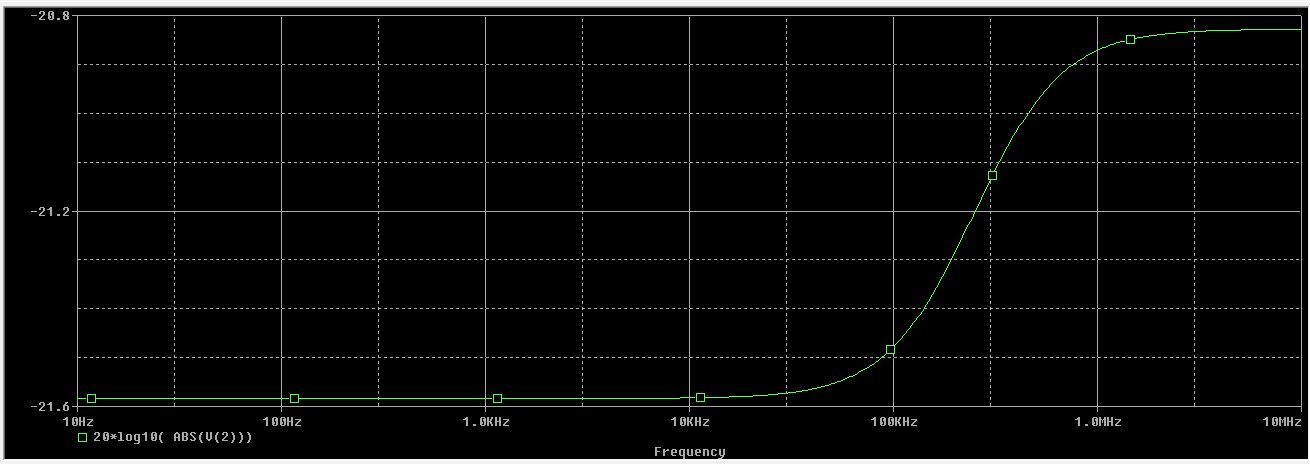
\includegraphics[width=5in]{Salida}
\caption{Barrido en Pspice}
\end{figure}

\textbf{Observación:}
El barrido en frecuencias encontró que cuando se llega a los -20dB, es decir a valores muy pequeños de voltaje es a frecuencias muy altas \\\\\\

Gráfica de los valores obtenidos con el barrido en frecuencia en el laboratorio:
\begin{figure}[h!]
\centering
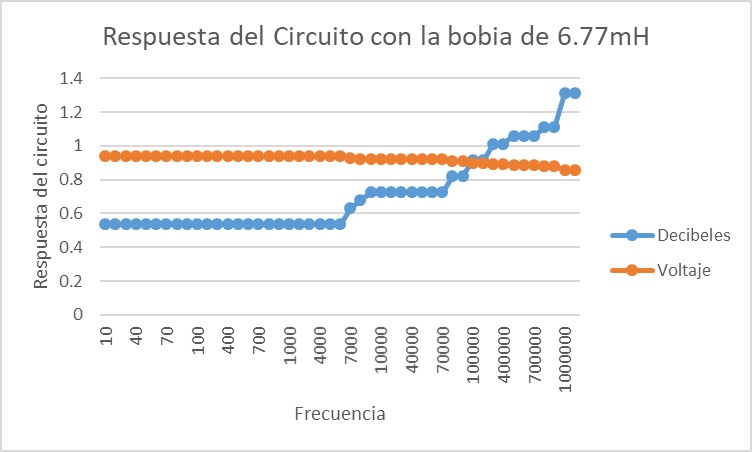
\includegraphics[width=5in]{Grafica}
\caption{Respuesta en el barrido de frecuencias del circuito}
\end{figure}

Tabla de los valores obtenidos en las mediciones del laboratorio:
\begin{figure}[h!]
\centering
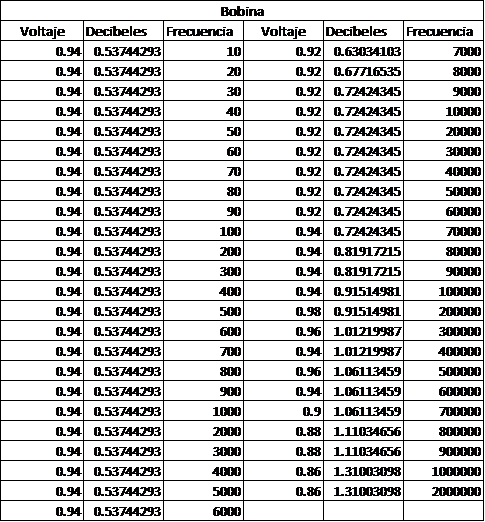
\includegraphics[width=5in]{Tab}
\caption{Valores obtenidos del barrido de frecuencias}
\end{figure}

\newpage
Respuesta a la función escalón con la función de Scilab.
\begin{figure}[h!]
\centering
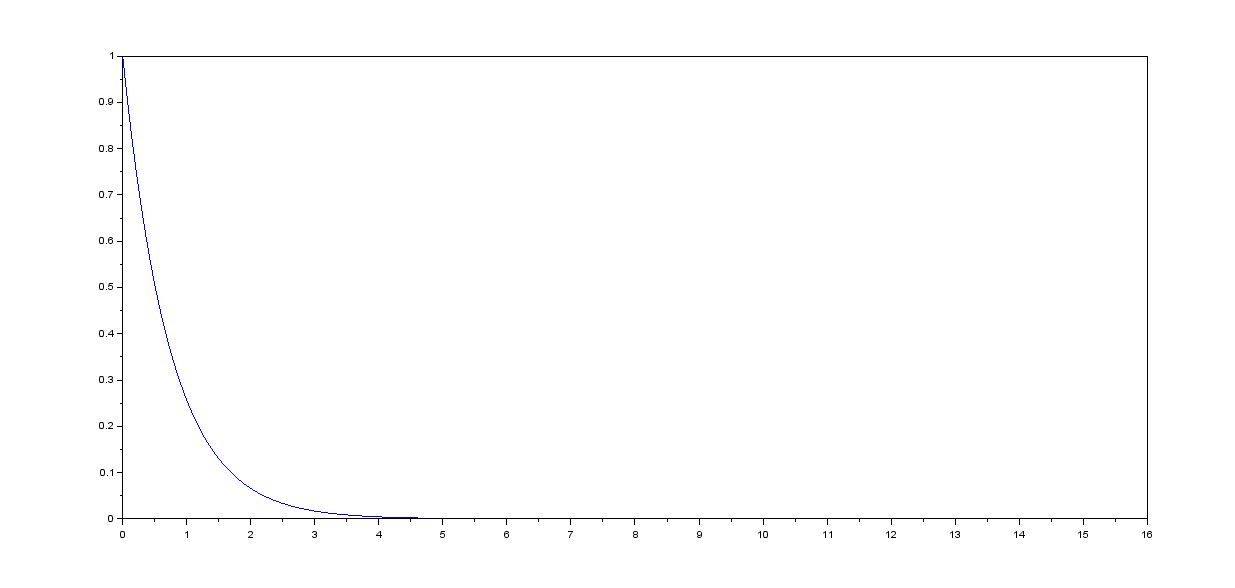
\includegraphics[width=5in]{G}
\caption{Respuesta en tiempo con el código de Scilab}
\end{figure}

Checar el tiempo de respuesta del circuito físico en el laboratorio.\\
\begin{figure}[h!]
\centering
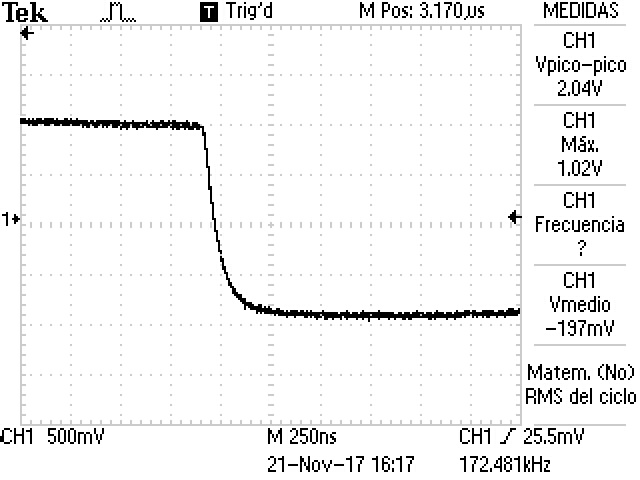
\includegraphics[width=5in]{TEK0044}
\caption{Respuesta en tiempo}
\end{figure}

\textbf{Observación:}
Se obtuvo un voltaje para encontrar el 63\% de la descarga de una función escalón, para encontrar la tau del inductor, el valor al que se encontró Tau fue a los 0.73V con un tiempo de 80nS, mediante la siguiente ecuación:\\\\
\begin{equation}\label{eq:ej11}
V(t)=\frac{V_{i}}{e}=\frac{2Vpp}{e}=0.7357V
\end{equation}
\newpage


%%%%%%%%%%%%%%%%%%%%%%%
\section{Conclusiones}
Martha Yepez Chavez:\\
Para realizar esta práctica previamente se realizaron los cálculos de la bobina y el inductor respectivamente, con sus simulaciones para poder comparar con los resultados obtenidos en laboratorio y verificar que la respuesta fuera la correcta. Para poder visualizar las raíces y los ceros de una función de transferencia se hizo uso  del plano complejo (Plano ‘s’). El otro uso del plano ‘s’ es el criterio de estabilidad de Nyquist, que permite determinar la estabilidad de un sistema de control mediante la inspección del diagrama de Nyquist de la respuesta de fase de la función de transferencia en el plano complejo. En esta práctica el diagrama de bode nos permitió caracterizar la respuesta en frecuencia de los sistemas analizados. Al concluir la práctica pudimos corroborar que los datos obtenidos prácticamente, coincidían con lo simulado previamente.
\\\\
Luz Vanessa Pacheco Medina:\\
La función característica del sistema eléctrico desarrollado en la práctica está dada por la función de transferencia, que es la salida entre la entrada del sistema, Las raíces del denominador son denominadas los polos de la función de transferencia, mientras que las raíces del numerador son denominados los ceros de la función de transferencia.
Las raíces de la ecuación característica, que son los polos de la función de transferencia, deben ser reales o deben ser pares complejos conjugados, una de las características para determinar la estabilidad del sistema es que las partes reales de todos los polos deben ser negativas para que el sistema sea estable, o de otra manera, que los polos se ubiquen del lado izquierdo del plano S, de Laplace.
Una de las formas para obtener la ecuación de trasferencia, de una forma visible para obtener los polos y ceros es por inspección, siendo una forma fácil de hacerlo, sin embargo, con las técnicas de análisis de circuitos tradicionales se obtiene el mismo resultado, pero se tiene que llevar a la forma de polos y ceros para encontrarlos fácilmente.
La respuesta en el tiempo del circuito con la bobina tiene un punto en el sube su valor según el diagrama de bode, ya que disminuye su voltaje a la salida, sin embargo, inicia con valores altos y termina con valores pequeños. De igual forma en la simulación responde de la misma forma el barrido la gráfica, pero en el implementado en el laboratorio no llega hasta los 10MHz que indica la simulación en Pspice sino sólo a 2MHz que son los que nos da el generador del laboratorio, por lo que el circuito no llegó hasta los -20dB a los que teóricamente se llegarían. 


%%%%%%%%%%%%%%%%%%%%%%%


%%%%%%%%%%%%%%
% Bibliografía
%%%%%%%%%%%%%%

\newpage

El formato recomendado para la bibliografía es el APA. El siguiente es un ejemplo:

\begin{thebibliography}{}
\bibitem[Apuntes, 2012]{Funciones de transferencia} \emph{http://ocw.uc3m.es/ingenieria-de-sistemas-y-automatica/senales-y-sistemas/temas/tema-4-funcion-de-transferencia} consultado el 26/10/2017.

\bibitem[Ingeniería de control moderna, 1998]{} Katsuhiko Ogata (1974). \emph{Ingeniería de control moderna}. USA:  Pearson Prentice Hall, 4th Edition.



\end{thebibliography}

\newpage


%%%%%%%%%%%%%%
\end{document}
%%%%%%%%%%%%%%
